%%%%%%%%%%%%%%%%%%%%%%%%%%%%%%%%%%%%%%%%%%%%
% Final version of Field Methods
% Last edits: Aug 4, 2016
%%%%%%%%%%%%%%%%%%%%%%%%%%%%%%%%%%%%%%%%%%%%

\documentclass[12pt]{article}
\usepackage{natbib}
\usepackage[letterpaper, margin=1.1in]{geometry}
\usepackage{graphicx}
\usepackage{wrapfig}
\usepackage{enumitem}
\setlist[enumerate]{itemsep=0mm}
\usepackage{multirow}
\usepackage{lscape}
\usepackage{caption}
\usepackage{subcaption}
\usepackage{hyperref}

\begin{document}
\noindent{Alexandra Pulwicki \\ \today}

\begin{center}
\Large \textbf{Field Methods and Report \\ May 2016}
\end{center}


\section*{Overview}

A winter snow survey was conducted on three glaciers in the Donjek Range of the St. Elias Mountains in May 2016. This report documents the field design and planning and how the planned work was implemented in the field.

***Still needed: close up photo of swe tube, snowpit cut outs?

\tableofcontents
\pagebreak

%%%%
\section{Field Design}
%%%%

\subsection{Sampling Scheme and Naming System}

Three glaciers within the Donjek Range were chosen as study sites and can be seen in Figure \ref{studysites}. Glaciers in the Donjek Range are unnamed but working names have been employed by \cite{Crompton2016} and are adopted for this work. Glacier 4, Glacier 2, and Glacier 13 were selected. These glaciers were chosen because these glaciers are spread throughout the Donjek Range and are located increasingly further from the large-scale topographic divide (located at the head of the Kaskawalsh Glacier \citep{Taylor1969}). The three glaciers are also located on different sides of the range-scale topographic divides, which run roughly from west to east in the southern area and from south to north in the eastern area and form an `L' shape. Glacier 4 is located on the southern side of the first arm, Glacier 2 is located on the northern side of the first arm and the western side of the second arm, and Glacier 13 is located on the eastern side of the second arm. The selected glaciers also have similar orientations and one central glacier-filled valley (similar shape). Within the Donjek Range, these glaciers have good SPOT5 DEM coverage, which provides the highest resolution DEM available for this area. Additionally, the majority of the three glaciers is accessible on foot and the total area is small enough (see Table \ref{glacierstats}) to allow for reasonable coverage using point measurements.

\begin{table}[b!]
\centering
\caption{Area, length, and elevation descriptors of three chosen glaciers.}
\label{glacierstats}
\begin{tabular}{|l|c|c|ccc|}
\hline
\multicolumn{1}{|c|}{} & \multirow{2}{*}{\textbf{Area (km$^2$)}} & \multirow{2}{*}{\textbf{Length (km)}} & \multicolumn{3}{c|}{\textbf{Elevation (m)}}         \\
\multicolumn{1}{|c|}{} &                                         &                                       & \textbf{Minimum} & \textbf{Maximum} & \textbf{Mean} \\ \hline
Glacier 4              & 5.26                                    & 6.2                                   & 1573             & 2854             & 2321          \\
Glacier 2              & 6.91                                    & 7.4                                   & 1906             & 3098             & 2472          \\
Glacier 13             & 12.33                                   & 9.5                                   & 1775             & 3037             & 2434          \\ \hline
\end{tabular}
\end{table} 

The sampling scheme for each glacier was chosen to be similar so that comparison between glaciers could be done more readily. Each glacier was divided into the accumulation area, upper ablation area, and lower ablation area. In the accumulation area, a central snowpit location was chosen. Additionally, a series of approximately ten snow coring locations was chosen throughout the accumulation area. Steep sections and glacier margins were avoided. In both the upper and lower ablation area a number of linear and curvilinear transects were mapped, which included an `hourglass and circle' (Parr, C., 2016 personal communication) as well as a transverse (below the hourglass) and midline transect. The length and width of each transect was adjusted to span the full dimension of its corresponding area. Snowpit locations in the ablation area were chosen to be at the centre of each hourglass. An overview of the sampling design can be seen in Figure \ref{transect_planned}.

The full ablation area was also divided into seven zones of approximately equal elevation intervals. Three locations within each zone were then randomly selected for zigzag \citep{Shea2010} measurements (Figure \ref{zigzag_planned}) and the three locations were randomly labelled as different priorities. The goal was to complete one zigzag in each zone. If possible, the measurement would be completed at the `Priority A' location but if it was not possible due to dangerous conditions then the `Priority B' or `Priority C' locations would be chosen. This allowed for random locations to be used but with the flexibility to adjust locations in the field. SWE measurements would be taken within each zigzag, and at snowpit locations with the ablation area.  

The location of each snow depth and density measurement is imported into hand-held GPS devices (Garmin GPSMAP 64s) as a waypoint with a unique name. Points that are part of a transect have a name with the glacier number, the transect and area that the point belongs to, and a three-digit sequential number. The code for the transect area and type includes two letters. The first letter is either `A' for `accumulation area', `U' for `upper ablation area', or `L' for `lower ablation area'. The second letter indicates the transect type, with `H' for `hourglass', `T' for `transverse transect', `C' for `circle', and `M' for `midline'. For example, the name G04\_UM023 is the 23rd point on the Midline transect in the Upper ablation area of Glacier 4, and G13\_LC134 is the 134th point on the circle in the lower ablation area of Glacier 13. Other points that are not part of a transect also follow a similar naming convention. The snowpit locations use the code `SP' (e.g. G04\_LSP is the snowpit located in the lower ablation zone of Glacier 4) and the firn coring locations have the code `FC' and a two digit number (e.g. G02\_AFC04 is the fourth firn core location in the accumulation area of Glacier 2).

The zigzag points have a name with the glacier number, the zone that they were located in, the zigzag priority, and the vertex number. The zone and priority (A, B, C) are indicated by a `Z', then the zone number, and then an `A', `B', or `C'. The vertex number is indicated by a `ZZ' and then a sequential number. For example, the vertex labelled G02\_Z2C\_ZZ04 is on Glacier 2 in zone 2 and the fourth point of a priority C zigzag. The vertex labelled G13\_Z7A\_ZZ08 is on Glacier 13 in zone 7 and the eighth point of a priority A zigzag. An example of a zigzag sampling scheme can be seen in Figure \ref{zigzag_vertex}.

\begin{landscape}
\begin{figure}
	\centering
	\fbox{\includegraphics[height = 0.95\textwidth]{chosenglaciers.jpeg}}\\
	\caption{Study glaciers in the Donjek Range, Yukon (see inset). The topographic divide is shown as a dashed line.}
	\label{studysites}
\end{figure}

\begin{figure}
	\centering
	\fbox{\includegraphics[height = 0.95\textwidth]{Transects_planned.jpeg}}\\
	\caption{Target waypoints for snow depth transects, snow pits, and SWE measurements on three study glaciers.}
	\label{transect_planned}
	\end{figure}

\begin{figure}
	\centering
	\fbox{\includegraphics[height = 0.95\textwidth]{Zigzag_planned.jpeg}}\\
	\caption{Randomly assigned locations for zigzag measurements in the ablation area (divided into seven zones).}
	\label{zigzag_planned}
\end{figure}
\end{landscape}

\begin{figure}
	\centering
	\fbox{\includegraphics[height = 0.95\textwidth]{ZZ_vertex.jpeg}}\\
	\caption{Example of zigzag. Vertices are labelled and measurements are taken at random intervals along the dashed lines between vertices. The randomly chosen location of the SWE measurement is shown as a diamond.}
	\label{zigzag_vertex}
\end{figure}


\subsection{Waypoint Creation and Upload to GPS Device}

To create the desired \textbf{transect} waypoints and enter them into the handheld GPS devices (Garmin GPSMAP 64s) the following steps were taken:
\begin{enumerate}
\item In QGIS, the outline of the glacier was selected from the Randolph Glacier Inventory (RGI 5.0) \citep{Pfeffer2014} and a recent, end-of-summer Landsat image was downloaded (LC80620172013248LGN00 image courtesy of the U.S. Geological Survey). 
\item The ELA was estimated by tracing out the snow line from the Landsat image.
\item The desired transects were traced out in QGIS within the intended area. The tool `QChainage' was then used to divide the line into points that were spaced every 30 m. Note that the shape file of the transect lines was projected into UTM coordinates to space points using units of metres. 
\item The new point file was then saved as a comma-separated value file (`.csv') and opened in Excel. Note that the projection of the file was WGS84 so that the exported file had latitude and longitude values, which were needed for the GPS software.
\item The points were then named according to their location, area, transect, and point order. A column was made for `Glacier' and `Transect' and filled in for each point (using the drag function in Excel). This required identifying the range of points in QGIS (which were numbered) that corresponded to each transect and relating them to the numbered points in the Excel file (this was a bit cumbersome). The two columns were then combined and a sequential number added to the end. This column requires the header 'name' to be correctly identified as the name of the point in the GPS software.
\item The file with the point names was then imported into to the Garmin software \textit{BaseCamp} and the waypoints were transferred to the GPS devices using this software. 
\end{enumerate}

To create the desired \textbf{zigzag} waypoints and enter them into the GPS devices the following steps were taken:
\begin{enumerate}
\item As described above, the outline of the glacier was selected from the RGI and a recent, end-of-summer Landsat image was downloaded. The ELA was estimated by tracing out the snow line from the Landsat image.
\item The ablation area was then divided into 7 zones that had approximately equal area (estimated by eye) and a polygon was traced out for each zone (within one shape file). 
\item In QGIS, the tool `Random Points' was then used to choose three random locations in each polygon. This was the location of the SWE measurements A, B, and C in each zone. 
\item The file with the SWE measurement locations was saved as a `.csv'. The points were then named in Excel and exported to the GPS device as described above.
\item A new shape file was then created for the vertices of the zigzag. The vertices were created (in sequential order) so that they fit along the edges of one cell of the SPOT5 DEM. This was done by actually looking at one cell and placing the points along the edges at the intended locations. As a result, the SWE measurement location within the zigzag was not the same between zigzags. 
\item Once all the zigzag point groups were created, the file was saved as a `.csv', points named accordingly, and then exported to the GPS device as described above. 
\end{enumerate}

The locations of snowpits and snow cores were chosen by hand in a separate shape file. This file was then saved as a `.csv', the points named, and the file exported to the GPS devices as described above. 

The files that had the names of the points were then imported back into QGIS so that the maps with point labels could be created.  Since the order of completing measurements was determined in the field, these maps helped to quickly decide on the most efficient plan because they aided in determining the relative location of zigzags and transects.

%%%%
\section{Implementation}
%%%%

\subsection{Linear and Curvilinear Transects}
\label{sec:transects}

The transects, which include the hourglass, circle, transverse transect, and midline, were all executed in a similar way. Along each transect, waypoints were marked every 30 m. To sample these locations, a team of four people was used in the configuration shown in Figure \ref{photo_probing} and schematically in Figure \ref{probing}. The four people were roped together so that during typical glacier travel there was approximately 10 m separating each person (likely ranged between 9.5 and 11 m). The front person was responsible for navigation and waypoint marking and would follow these steps for each measurement location:
\begin{enumerate}
\item Use the GPS device to locate each intended waypoint
\item Navigate to that location using the GPS device
\item Stop and inform the team when they had arrived at the location
\item Mark a new waypoint on the GPS device as the real location of the measurement (allow for auto labelling of waypoint, which was a three digit number that increased by one with subsequent waypoints). When needed, call out the waypoint label to the team.
\item In one line of a field book, write the labels `Intended' for the waypoint that was being navigated to (code created during planning stage), `Real' for the name of the newly created waypoint on the GPS device (three digit number), as well as the easting, northing, and elevation for that location. This served as the backup for locating measurement points in the event of GPS device failure. 
\end{enumerate}

The remaining three people took snow depth measurement using a graduated 3.2 m avalanche probe. Upon arriving at the waypoint they would follow these steps:
\begin{enumerate}
\item Insert the probe into the snow until the snow/ice interface was reached. Read the depth of the snow pack on the probe to 0.5 cm. Repeat two (or three) more times (total of three (or four) measurements) within a 1 m$^2$ area of the first measurement and in a way that the three (or four) measurements are approximately equidistant. 
\item In one line of a field book, record the `Real' waypoint label (three digit number), as well as the three (or four) depth measurements. 
\end{enumerate}
Note that the snow/ice interface could often be differentiated from an ice lens. Typically, glacier ice felt hard, had a thin, low density (empty feeling) layer above, and created a bright `ping' sound in the probe. Ice lenses felt sticky and the probe would make a dull `thud' sound. In some locations this differentiation was obvious while in other locations it was difficult to be determine what was at the end of the probe. Often, layers in the snowpack could be felt with the probe. For example, the probe would move easily through low density layers such as depth hoar and would `stick' to hard layers or ice lenses. Increasing the force applied to the probe would usually allow the probe to penetrate through hard layers. In cases where the `sticky' layer could not be penetrated, the observer would place a question mark next to the recorded depth or simply omit that measurement. A question mark was also placed beside measurements that were notably smaller than adjacent measurements, which suggested much deeper snow. Note that the probe was inserted vertically, which was not necessarily perpendicular to the snow surface.

It was originally planned for each observer to take four depth measurements in a square pattern. However, during the first transect the observers found time consuming and difficult to remember and record four depths. The observers found that the most efficient way to collect data was to take three depth measurements, remember the values, and then write them all down in the field book. When four measurements were taken it was too difficult to remember all the values simultaneously so the whole process would take much longer. The decision was made to decrease the number of measurements so that we could increase the number of locations measured. 

There were dedicated field books for each type of measurement rather than each observer. The first person had the `Navigation' field book, the second person had `Snow depth \#1', the third person had `Snow depth \#2', and the fourth person had `Snow depth \#3'. In this way, the location of each measured value can be inferred from its location relative to the navigation person (where the location was being recorded). For example, the `Snow depth \#3' value was located $\sim$30 m behind the waypoint location along the trajectory between the previous and current waypoint. This arrangement was preferred to having a field book for each observer because it minimized confusion and potential errors when entering and processing data.

In this arrangement, snow depth measurements could be taken every 10 m along a transect if a waypoint was marked every 30 m. For the first two transects, measurements were completed at every waypoint. However, this also proved to be too time consuming so measurements were taken at every second waypoint for subsequent transects (exceptions include the midline on Glacier 4 and the lower hourglass on Glacier 2, see Table \ref{tab:snowdepthsummary}). A schematic of this arrangement can be seen in Figure \ref{probing:mapview}. Waypoints that were too dangerous to access were omitted. Additional waypoints (not originally uploaded to GPS devices) were created in some instances when travelling from the last accessible waypoint to the next accessible waypoint. A summary of information about the completed snow depth transects can be seen in Table \ref{tab:snowdepthsummary}.

\begin{figure}
	\centering
	\fbox{\includegraphics[width = 0.95\textwidth]{photo_probing.jpg}}\\
	\caption{Implementation of transect probing. The first person navigated to the intended waypoint using the GPS device. The second, third, and fourth (not seen) observers are probing using 3.2 m long avalanche probes. There is approximately 10 m between observers. Photo credit: G. Flowers}
	\label{photo_probing}
	\end{figure}


\begin{figure}
    \centering
    \begin{subfigure}[b]{0.8\textwidth}
        \fbox{\includegraphics[width=\textwidth]{probers1.jpg}}
        \caption{Relative location of four people taking depth measurements at desired locations.}
        \label{probing:people}
    \end{subfigure}
    
    \begin{subfigure}[b]{0.8\textwidth}
        \fbox{\includegraphics[width=\textwidth]{probers2.jpg}}
        \caption{Intended and actual transect depth measurement spacing. In the intended design, there was continuous measurement with 10 m sampling interval. In the actual implementation, every second waypoint was accessed so there was 60 m between subsequent measurements.}
        \label{probing:mapview}
    \end{subfigure}

    \caption{Schematic of the snow depth measurement configuration. Blue circles indicate depth measurement and orange squares indicate waypoint (WP) location.}\label{probing}
\end{figure}

\begin{landscape}

\begin{table}[]
\footnotesize
\centering
\caption{Summary information for snow depth transects. Transect shapes completed include Lower Hourglass (LH), Lower Circle (LC), Lower Midline (LM), Upper Hourglass (UH), Upper Circle (UC), Upper Midline (UM), Upper Transect (UT), and Bonus Transect (BT). The first observer was navigating to waypoints and the remaining three were taking depth measurements.}
\label{tab:snowdepthsummary}
\begin{tabular}{ccccccl}

\textbf{Glacier}                                                             & \textbf{Shape}                                               & \textbf{\begin{tabular}[c]{@{}c@{}}Measurement\\ Interval\end{tabular}}  & \textbf{Date} & \textbf{\begin{tabular}[c]{@{}c@{}}GPS \\ Waypoint\\  Labels\end{tabular}} & \textbf{\begin{tabular}[c]{@{}c@{}}Observer\\  Order\end{tabular}} & \multicolumn{1}{c}{\textbf{Comments}}                                                                                                                                                                                                            \\ \hline
\multirow{7}{*}{\begin{tabular}[c]{@{}c@{}}Glacier 4\\ (G04)\end{tabular}}   & \textbf{LH}                                                  & \begin{tabular}[c]{@{}c@{}}30 m \\ (60 m for \\ upper part)\end{tabular} & 4 May 2016    & 021 -- 070                                                                 & GF--AP--CA--AC                                                     & \begin{tabular}[c]{@{}l@{}}4 depth measurement/location \\ along upper part\end{tabular}                                                                                                                                                         \\
                                                                             & \textbf{LC}                                                  & 60 m                                                                     & 6 May 2016    & 159 -- 184                                                                 & GF--AP--CA--AC                                                     &                                                                                                                                                                                                                                                  \\
                                                                             & \textbf{LM}                                                  & 90 m                                                                     & 7 May 2016    & 185 -- 207                                                                 & AP--GF--CA--AC                                                     &                                                                                                                                                                                                                                                  \\
                                                                             & \textbf{UH}                                                  & 60 m                                                                     & 5 May 2016    & 072 -- 126                                                                 & CA--GF--AP--AC                                                     &                                                                                                                                                                                                                                                  \\
                                                                             & \textbf{UC}                                                  & 60 m                                                                     & 5 May 2016    & 127 -- 157                                                                 & CA--GF--AP--AC                                                     &                                                                                                                                                                                                                                                  \\
                                                                             & \textbf{UM}                                                  & 90 m                                                                     & 7 May 2016    & 208 -- 221                                                                 & AP--GF--CA--AC                                                     & Additional measurement at WP 158 (6 May 2016)                                                                                                                                                                                                               \\
                                                                             & \textbf{UT}                                                  & 30 m                                                                     & 4 May 2016    & 004 -- 020                                                                 & GF--AP--CA--AC                                                     & 4 depth measurement/location                                                                                                                                                                                                                     \\ \hline
\multirow{7}{*}{\begin{tabular}[c]{@{}c@{}}Glacier 2 \\ (G02)\end{tabular}}  & \textbf{\begin{tabular}[c]{@{}c@{}}LH \\ \& LC\end{tabular}} & 30 m                                                                     & 11 May 2016   & 371 -- 518                                                                 & GF--AP--CA                                                         & \begin{tabular}[c]{@{}l@{}}Only two probers. Avoided crossing main \\ channel so LH \& LC were combined and \\ done together on glacier right and then \\ glacier left of the channel. Almost all \\ measurements in the dune area.\end{tabular} \\
                                                                             & \textbf{LM}                                                  & $\sim$60 m                                                               & 10 May 2016   & 355 -- 370                                                                 & AP--GF--CA--AC                                                     & \begin{tabular}[c]{@{}l@{}}Original points along supraglacial stream \\ bed so points moved to glacier right and \\ locations were approximated\end{tabular}                                                                                     \\
                                                                             & \textbf{UH}                                                  & 60 m                                                                     & 8 May 2016    & 223 -- 275                                                                 & AC--AP--CA--GF                                                     & \begin{tabular}[c]{@{}l@{}}Many corner points avoided due to \\ crevasse danger\end{tabular}                                                                                                                                                     \\
                                                                             & \textbf{UC}                                                  & 60 m                                                                     & 8 May 2016    & 276 -- 313                                                                 & AC--AP--CA--GF                                                     &                                                                                                                                                                                                                                                  \\
                                                                             & \textbf{UM}                                                  & 60 m                                                                     & 9 May 2016    & 313 -- 343                                                                 & AC--AP--CA--GF                                                     &                                                                                                                                                                                                                                                  \\
                                                                             & \textbf{UT}                                                  & 60 m                                                                     & 11 May 2016   & 519 -- 528                                                                 & GF--AP--CA                                                         & Only two probers                                                                                                                                                                                                                                 \\
                                                                             & \textbf{BT}                                                  & $\sim$60 m                                                               & 19 May 2016   & 344 -- 354                                                                 & GF--AP--CA--AC                                                     &                                                                                                                                                                                                                                                  \\ \hline
\multirow{7}{*}{\begin{tabular}[c]{@{}c@{}}Glacier 13 \\ (G13)\end{tabular}} & \textbf{LH}                                                  & 60 m                                                                     & 15 May 2016   & 745 -- 811                                                                 & AC--AP--CA--GF                                                     &                                                                                                                                                                                                                                                  \\
                                                                             & \textbf{LC}                                                  & 60 m                                                                     & 15 May 2016   & 812 -- 847                                                                 & AC--AP--CA--GF                                                     &                                                                                                                                                                                                                                                  \\
                                                                             & \textbf{LM}                                                  & 60 m                                                                     & 14 May 2016   & 714 -- 743                                                                 & AC--AP--CA--GF                                                     &                                                                                                                                                                                                                                                  \\
                                                                             & \textbf{UH}                                                  & 60 m                                                                     & 12 May 2016   & 571 -- 650                                                                 & AC--GF--CA--AP                                                     &                                                                                                                                                                                                                                                  \\
                                                                             & \textbf{UC}                                                  & 60 m                                                                     & 12 May 2016   & 529 -- 570                                                                 & AC--GF--CA--AP                                                     &                                                                                                                                                                                                                                                  \\
                                                                             & \textbf{UM}                                                  & 60 m                                                                     & 14 May 2016   & 678 -- 713                                                                 & AC--AP--CA--GF                                                     &                                                                                                                                                                                                                                                  \\
                                                                             & \textbf{UT}                                                  & 60 m                                                                     & 14 May 2016   & 660 -- 677                                                                 & AC--AP--CA--GF                                                     &                                                                                                                                                                                                                                                 
\end{tabular}
\end{table}

\normalsize
\begin{table}[]
\centering
\caption{Summary information for zigzag measurements}
\label{tab:zigzagsummary}
\begin{tabular}{cccccl}
\textbf{Glacier} & \textbf{Zone} & \textbf{Priority} & \textbf{Date} & \textbf{Observers} & \multicolumn{1}{c}{\textbf{Comments}}                                                                          \\ \hline
G04              & 3             & A                 & 5 May 2016    & AP/CA              &                                                                                                                \\
G04              & 2             & A                 & 7 May 2016    & CA/AC              &                                                                                                                \\
G04              & 5             & B                 & 7 May 2016    & AP/GF              & \begin{tabular}[t]{@{}l@{}}Sticky layer - many points not collected\\ Snowing during measurements\end{tabular} \\ \hline
G02              & 5             & C                 & 10 May 2016   & CA/GF              & \begin{tabular}[t]{@{}l@{}}Extra line measured\\ Vertex labelling error in GPS device \end{tabular}                                                                                   \\
G02              & 7             & A                 & 10 May 2016   & CA/GF/AP/AC              & \begin{tabular}[t]{@{}l@{}}Channel present\\ Vertex labelling error in GPS device\end{tabular}                        \\
G02              & 3             & B                 & 10 May 2016   & GF/AP              & Vertex labelling error in GPS device                                                                                  \\ \hline
G13              & 7             & C                 & 14 May 2016   & AC/AP              & Vertex labelling error in GPS device                                                                                  \\
G13              & 4             & C                 & 14 May 2016   & GF/CA              & \begin{tabular}[t]{@{}l@{}}Channel present\\ Vertex labelling error in GPS device\end{tabular}                        \\
G13              & 3             & B                 & 15 May 2016   & GF/CA              & Vertex labelling error in GPS device                                                                                  \\
G13              & 5             & A                 & 15 May 2016   & AP/AC              & \begin{tabular}[t]{@{}l@{}}Mushy snow that collapses\\ Vertex labelling error in GPS device\end{tabular}             
\end{tabular}
\end{table}

 \begin{figure}
	\centering
	\fbox{\includegraphics[height = \textwidth]{zigzag_completed.png}}\\
	\caption{Snow depth values measured along a zigzag pattern (G04\_Z3A)}
	\label{zigzag_example}
\end{figure}

\end{landscape}

\begin{table}[]
\centering
\caption{Summary information for SWE measurements with the Federal Snow Sampler}
\label{tab:SWEsummary}
\begin{tabular}{ccccccl}
\textbf{Glacier}      & \textbf{Location} & \textbf{\begin{tabular}[c]{@{}c@{}}Total\\ Values\end{tabular}} & \textbf{\begin{tabular}[c]{@{}c@{}}Number \\ of Tube \\ Lengths\end{tabular}} & \textbf{Date} & \textbf{Observers} & \multicolumn{1}{c}{\textbf{Comments}}                                        \\ \hline
\multirow{7}{*}{G04}  & Z3A               & 5                                                               & 3                                                                             & 5 May 2016    & GF/AC              &                                                                              \\
                      & USP               & 2+2+2+3                                                         & 3                                                                             & 5 May 2016    & GF/CA              &                                                                              \\
                      & Z2A               & 3                                                               & 3                                                                             & 7 May 2016    & GF/AP              &                                                                              \\
                      & LSP               & 3+2+2+2                                                         & 3                                                                             & 7 May 2016    & GF/CA              &                                                                              \\
                      & Z5B               & 3                                                               & 3                                                                             & 7 May 2016    & CA/AC              &                                                                              \\
                      & Z5A               & 3                                                               & 3                                                                             & 7 May 2016    & CA/AC              &                                                                              \\
                      & Z5C               & 3                                                               & 2                                                                             & 7 May 2016    & CA/AC              &                                                                              \\ \hline
\multirow{7}{*}{G02}  & Z5C               & 3                                                               & 2                                                                             & 10 May 2016   & AP/AC              &                                                                              \\
                      & USP               & 3+2+2+2                                                         & 2                                                                             & 10 May 2016   & AP/AC              &                                                                              \\
                      & Z7A               & 3                                                               & 3                                                                             & 10 May 2016   & CA/GF              &                                                                              \\
                      & Z7B               & 3                                                               & 3                                                                             & 10 May 2016   & CA/GF              &                                                                              \\
                      & Z7C               & 3                                                               & 2                                                                             & 10 May 2016   & AP/CA              &                                                                              \\
                      & LSP               & 2+2+2+2                                                         & 1                                                                             & 10 May 2016   & CA/AC              & \begin{tabular}[t]{@{}l@{}}Used snowpit \\ spring scale (grams)\end{tabular} \\
                      & Z3B               & 3                                                               & 1                                                                             & 10 May 2016   & CA/AC              & \begin{tabular}[t]{@{}l@{}}Used snowpit \\ spring scale (grams)\end{tabular} \\ \hline
\multirow{19}{*}{G13} & ASP               & 2+2+2+2                                                         & 3                                                                             & 13 May 2016   & AP/AC              &                                                                              \\
                      & AFC05             & 3                                                               & 3                                                                             & 13 May 2016   & AP/CA              & \begin{tabular}[t]{@{}l@{}}Probe depth \\ $\neq$ tube depth\end{tabular}     \\
                      & WP 651            & 3                                                               & 3                                                                             & 13 May 2016   & AP/CA/GF           &                                                                              \\
                      & WP 652            & 4                                                               & 3                                                                             & 13 May 2016   & AP/CA/GF           &                                                                              \\
                      & WP 653            & 3                                                               & 3                                                                             & 13 May 2016   & AP/CA/GF           &                                                                              \\
                      & WP 654            & 3                                                               & 3                                                                             & 13 May 2016   & AP/CA/GF           &                                                                              \\
                      & WP 655            & 3                                                               & 3                                                                             & 13 May 2016   & AP/CA/GF           &                                                                              \\
                      & WP 656            & 3                                                               & 3                                                                             & 13 May 2016   & AP/CA/GF           &                                                                              \\
                      & WP 657            & 3                                                               & 3                                                                             & 13 May 2016   & AP/CA/GF           &                                                                              \\
                      & WP 658            & 3                                                               & 3                                                                             & 13 May 2016   & AP/CA/GF           &                                                                              \\
                      & WP 659            & 3                                                               & 3                                                                             & 13 May 2016   & AP/CA/GF           &                                                                              \\
                      & Z7C               & 3                                                               & 2                                                                             & 13 May 2016   & CA/GF              &                                                                              \\
                      & USP               & 2+2+2+2                                                         & 2                                                                             & 14 May 2016   & AP/AC              & \begin{tabular}[t]{@{}l@{}}Ice layer near \\ bottom\end{tabular}             \\
                      & Z4C               & 3                                                               & 3                                                                             & 14 May 2016   & AP                 & In stream channel                                                            \\
                      & WP 744            & 3                                                               & 2                                                                             & 14 May 2016   & AP                 & In Z4C zigzag                                                                \\
                      & Z3B               & 3                                                               & 2                                                                             & 15 May 2016   & AP/AC              &                                                                              \\
                      & Z4B               & 3                                                               & 2                                                                             & 15 May 2016   & AP/AC              &                                                                              \\
                      & Z5C               & 3                                                               & 2                                                                             & 15 May 2016   & CA/GF              &                                                                              \\
                      & Z5B               & 3                                                               & 2                                                                             & 15 May 2016   & CA/AC              &                                                                             
\end{tabular}
\end{table}



\subsection{Zigzag}

The zigzag sampling pattern was used to obtain many measurements within a 40 x 40 m area.  The pattern consisted of two intersecting `Z' shaped transects. Snow depth was measured with random spacing between 0.3 m and 3.0 m. 

Two teams of two people were used to complete each zigzag. The first team would navigate to the vertices of the zigzag using the GPS device and place wands at each vertex. Often the tracks would not be straight between two vertices so the second team would use the wands to travel between vertices in as straight a line as possible. The first person would use the avalanche probe to measure out the distance to the next measurement spot and then probe at that point (Sturm, M., 2016 personal communication). Probing protocol was exactly the same as for transect measurements (see Section \ref{sec:transects}). The first person would call out the depth to the second person, who was responsible for recording the distance between measurements and the depth at the measurement point. A field book was dedicated to zigzag measurements and each page would have the name of the vertex where measurements started, the distance from the previous measurement point and the depth at that point. The second person also had a sheet with random numbers from a uniform distribution between 0.3 and 3.0 m (generated used Matlab) and would call out these numbers in order as the distance between measurement points. While the second team was measuring snow depth, the first team took three SWE measurements with a $\sim$1 m area around the predetermined location within the zigzag area (see Section \ref{sec:SWE} for protocol). An example of a completed zigzag pattern can be seen in Figure \ref{zigzag_example} and a summary of information about completed zigzags can be seen in Table \ref{tab:zigzagsummary}.


 \subsection{Federal Snow Sampler}
\label{sec:SWE}
 
\begin{figure}
    \centering
    \begin{subfigure}[b]{0.38\textwidth}
        \fbox{\includegraphics[width=\textwidth]{photo_swe1.JPG}}
        \caption{Inserting the Federal Sampler into the snow. Photo credit: C. Ariagno}
        \label{photo_swe1}
    \end{subfigure}
    ~
    \begin{subfigure}[b]{0.56\textwidth}
        \fbox{\includegraphics[width=\textwidth]{photo_swe2.jpg}}
        \caption{Weighing the Federal Sampler with snow core on the spring scale (units of cm SWE). Photo credit: G. Flowers}
        \label{photo_swe2}
    \end{subfigure}

    \caption{Using the Federal Sampler to measure SWE}
    \label{photo_swe}
\end{figure}
 
A metric Federal Snow Sampler from Geo Scientific Ltd. was used to measure snow depth and snow water equivalent (SWE). At the predetermined locations, three measurements (within 50 cm of each other) were made using the sampler. At the snowpit locations, a total of eight measurements were made, with two measurements on each side of the snowpit. Density calculated from these values will be compared with density determined from sampling within the snow pit (see Section \ref{sec:snowpit}). 

The Federal Snow Sampler consists of four 0.83 m sections that could be screwed together. One end of the sampler has cutter teeth and the other end has a removable thread protector that can be screwed onto the top section of the tube. The sampler has graduations in units of 1 cm and slits along the side of the tube allow the observer to determine the length of the core when it is in the tube. The spring scale that comes with the Federal Sampler is in units of cm SWE.  

To take a measurement with the Federal Sampler the following steps were taken:
\begin{enumerate}
\item Three depth measurements (within $\sim$50 cm of each other) were made using an avalanche probe and the depths were recorded.
\item The weight (in cm SWE) of the assembled empty tube was measured using the spring scale and then recorded (tare).
\item The tube was placed vertically into the snow and then pushed and twisted clockwise so that the cutters at the end of the tube would penetrate the snow pack. If this proved to be too difficult, the T-handle was added onto the tube to aid in pushing the tube further into the snow. 
\item When the bottom of the snow pack was reached, the observer would measure the snow depth by using the graduation on the outside of the tube.
\item The tube was then gently pulled out of the snow (so as not to lose any snow from the bottom). The length of the snow core inside the tube was then measured by using the side slits to see the top of the core and lining it up with the graduation on the outside of the tube. This value was then recorded. If the length of the snow core was much less than the snow depth (typically a result of lost snow), the sample measurement was redone.
\item The snow and tube were weighed together using the spring scale and the value was recorded.
\item The tube was then emptied and wiped using a soft cloth on a pole to remove any moisture. 
\end{enumerate}

When the T-handle was used, the tube segments often became difficult to take apart. The small handles provided in the kit aided in disassembling the Federal Sampler. However, if a significant force was applied to the T-handle during sampling and the tube segments seized then longer handles (accomplished by attaching snow shovel handles to provided tools) helped in disassembling the sampler. Anti-seizing compound was included in the kit and was applied when needed. A summary of information about completed SWE measurements can be seen in Table \ref{tab:SWEsummary}.

\subsection{Firn Corer}

The firn corer was intended to be used in the accumulation area to extract a snow/firn core. The coring device would be beneficial in the accumulation area because the core can be extracted and used to determine the location of the snow/firn transition. From that, the snow depth and the mass of the snow core, which included only the past year of accumulation, could be determined. The Federal Sampler was thought to be ineffective in the accumulation area because the snow/firn transition may not have been felt and the core cannot be examined to establish where the transition occurs.

When the corer was used in the field however, a number of problems were encountered that prevented the collection of accurate measurements. The first was that the snow core would get stuck inside the core barrel. Warm temperatures meant that the barrel would get wet from snow melt and when it was inserted into the snow pack, the snow would freeze onto the side of the barrel. This meant that the core was destroyed in the extraction process. The second problem (which was connected to the first problem) was that the coring chips in the hole could not be discriminated from the core itself. Coring chips are loose snow crystals that fall to the bottom of the drilling hole when the barrel is taken out. When the barrel is reinserted for the second (or third) core, the snow in the subsequent core will contain these coring chips, which are not part of the intended core. The mass of the core will be incorrect (overestimate) because of this additional snow. This problem is typically avoided by extracting the in-tact core and identifying and removing the coring chips. However, since the core could not be extracted as one piece, this step was not possible and the masses of the cores were incorrect. 

In a few locations, sections of the core could be exacted without breaking them apart. In these areas the snow/firn transition could be identified. This means that in principal, the firn corer could be used to determine the depth of this transition. The main challenge is therefore being able to identify chips. In firn core trials that occurred after this field work, it was found that the the cores could be pulled out easily if the barrel was not totally full. However, in these less compacted cores the chips were difficult to identify so the problem persists. 

As a result of these complications, many accumulation area measurements on Glacier 4 and Glacier 2 were abandoned. On Glacier 13, the Federal Sampler was successfully used to take SWE measurements. The snow/firn transition could be felt with the Federal Sampler because of the large density change, which made it almost impossible to further insert the tube into the snow pack.  

\subsection{Snowpit}
\label{sec:snowpit}


Three snowpits were excavated on each glacier and snow density sampled every 10 cm using a wedge cutter (Snow Metrics RIP 2 Cutter (250 cc)). The snow temperature was also measured at 10 cm intervals. The snowpit was oriented so that the sampling face was in the shade (typically south edge of snowpit), which reduces melt. 

The measurement procedure in the snowpit was as follows:
\begin{enumerate}
\item The face of the wall that was chosen for sampling was smoothed and a ruler was placed against the wall with the 0 cm mark at the bottom of the snowpit. The ruler was used to measure sampling heights within the snow pack. The snow surface directly above this wall was undisturbed during the digging process so that the true snow depth could be determined. 
\item Air and snow surface temperature were measured by placing the thermometer (dial-stem thermometer ($\pm$0.5$^\circ$)) in the shade of a shovel or ski. 
\item A snow density sample was taken in 10 cm intervals through the full depth of the snow pack. Samples were offset horizontally from each other so that the snow was not affected by previous measurements. 
	\begin{enumerate}
	\item The wedge cutter was inserted into the snow vertically (to sample 10 cm intervals) and the top was slid onto the wedge to isolate the sample. The wedge was taken out and inspected. If the sample appeared to fill the entire wedge (no obvious voids) then the wedge was emptied into a small plastic bag. If the sample was poor then the snow was discarded and a new sample was taken at the same height in the snow pit. 
	\item A spring scale ($\pm$2.5 g) was then used to weigh the bag with the snow sample and the weight was recorded. The snow sample was then discarded. Note that the spring scale was tared with an empty bag.
	\end{enumerate}
\item Snow temperatures were also measured and recorded every 10 cm. The thermometer was inserted into the snow at the desired location and left to equilibrate for several minutes. The temperature was then recorded.
\end{enumerate}

Modifications to this procedure occurred when snow samples could not be taken because the snow was too dense. This would often occur when ice layers or lenses were present in the snow, which could not be cut by the wedge. In these cases, the measured thickness was recorded. A sample would then be taken using the wedge cutter but aligned horizontally so that a 5 cm tall sample was taken. Additionally, the sample interval closest to the ice surface (0--10 cm) would be difficult to obtain because the ice was rough and the snow above was faceted. Sometimes, this sample could not be obtained or a 5 cm sample needed to be taken. 

After the majority of snowpit measurements were completed, a spring scale with finer resolution was found. For Glacier 4 and 2 the coarse resolution (10 g) scale had been used but for Glacier 13 the fine resolution (2 g) scale was used. Future measurements should use the finer resolution spring scale when using the small wedge sampler. As a result, the snow-density uncertainty is larger for Glacier 4 and 2 than for Glacier 13. 

\begin{figure}
	\centering
	\fbox{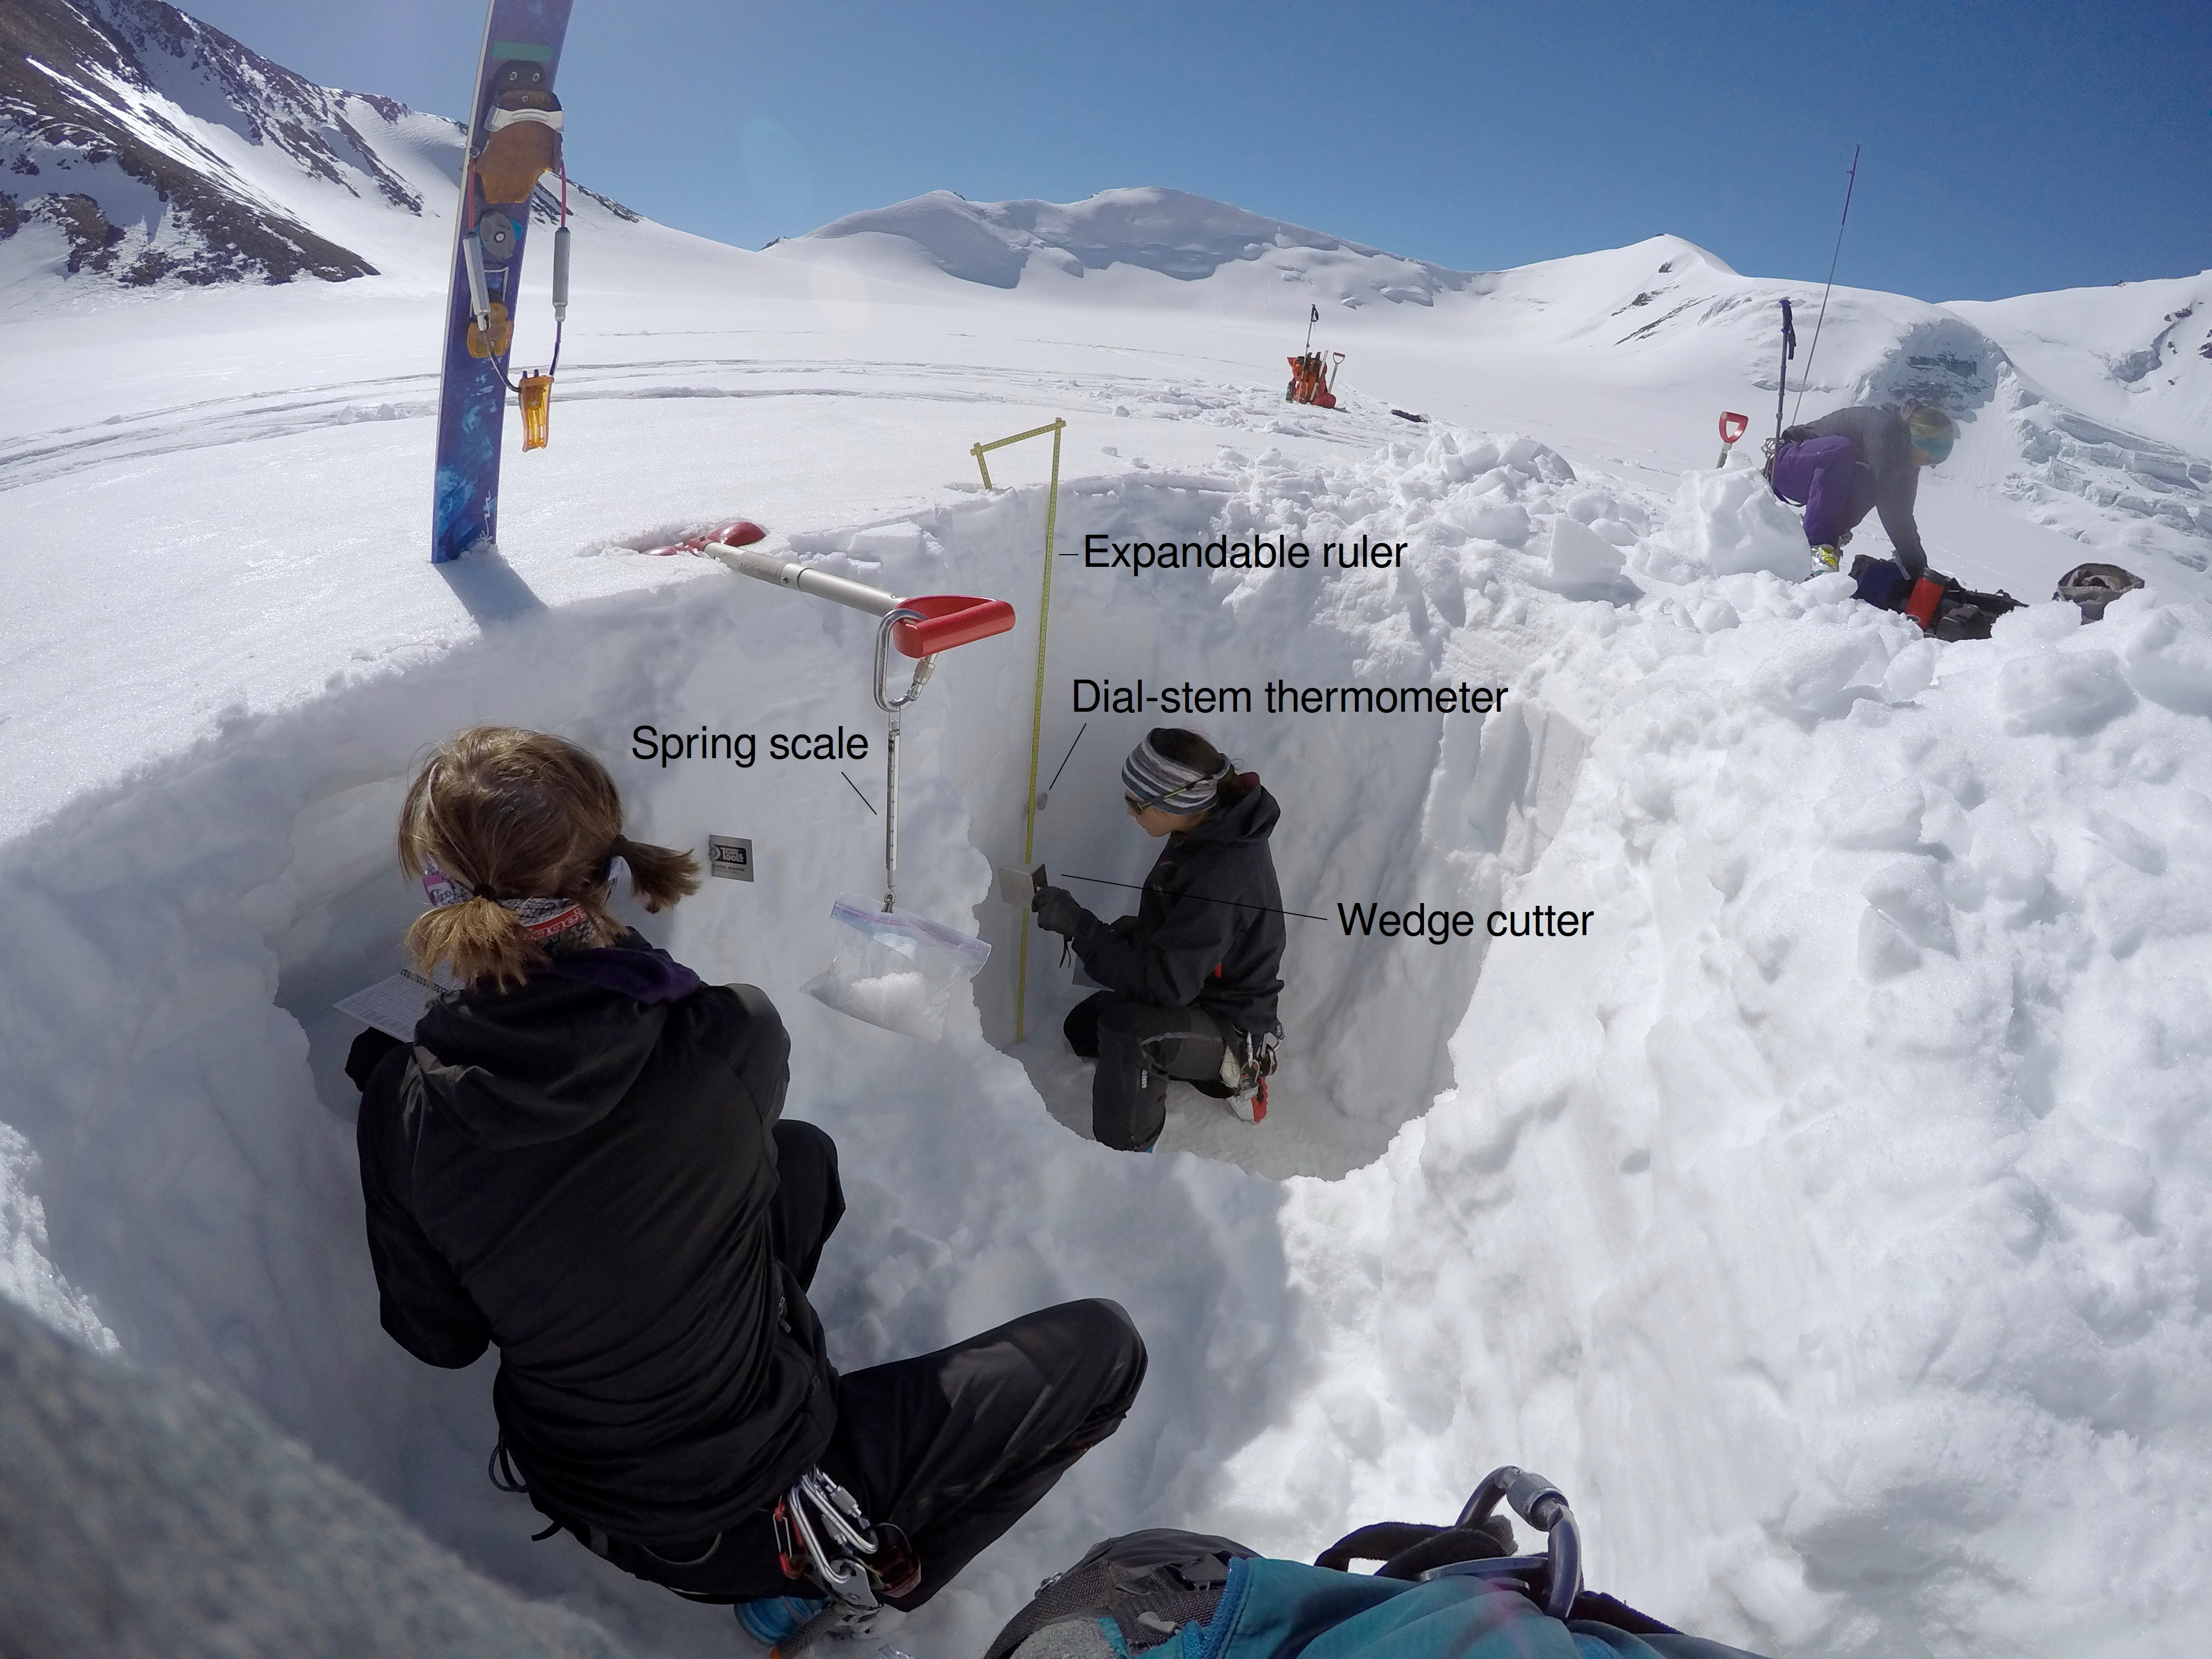
\includegraphics[width = 0.95\textwidth]{photo_snowpit.jpg}}\\
	\caption{Taking snow denisty measurements in a snowpit. An expandable ruler is used to measure snow depth and determine sampling locations. A 250cc wedge cutter is used to extract a known volume of snow and a spring scale is used to weigh the snow. The dial-stem thermometer is used for measureing snow temperature. Note that the sampling wall is shaded, has an undistrubed snow surface above it, and has a smoothed face. Photo credit: A. Criscitiello}
	\label{photo_snowpit}
	\end{figure}
	
%%%%%%%%

\bibliography{/home/glaciology1/Documents/MastersDocuments/MastersLit}
\bibliographystyle{igs}

\pagebreak
\section*{Appendix I - Field maps}

\noindent \large{\textbf{Glacier 4}}\\
\fbox{\includegraphics[height = 0.45\textheight]{G04_Topo.jpeg}}\\
\fbox{\includegraphics[height = 0.45\textheight]{G04_Overview.jpeg}}\\
\fbox{\includegraphics[height = 0.45\textheight]{G04_ZZ.jpeg}}\\
\fbox{\includegraphics[height = 0.45\textheight]{G04_LH.jpeg}}\\
\fbox{\includegraphics[height = 0.45\textheight]{G04_LH.jpeg}}\\
\fbox{\includegraphics[height = 0.45\textheight]{G04_UH.jpeg}}\\
\fbox{\includegraphics[height = 0.45\textheight]{G04_M.jpeg}}\\
\fbox{\includegraphics[height = 0.45\textheight]{G04_A.jpeg}}\\

\pagebreak
\noindent \large{\textbf{Glacier 2}}\\
\fbox{\includegraphics[height = 0.45\textheight]{G02_topo.jpeg}}\\
\fbox{\includegraphics[height = 0.45\textheight]{G02_Overview.jpeg}}\\
\fbox{\includegraphics[height = 0.45\textheight]{G02_ZZ.jpeg}}\\
\fbox{\includegraphics[height = 0.45\textheight]{G02_LH.jpeg}}\\
\fbox{\includegraphics[height = 0.45\textheight]{G02_LH.jpeg}}\\
\fbox{\includegraphics[height = 0.45\textheight]{G02_UH.jpeg}}\\
\fbox{\includegraphics[height = 0.45\textheight]{G02_M.jpeg}}\\
\fbox{\includegraphics[height = 0.45\textheight]{G02_A.jpeg}}\\

\pagebreak
\noindent \large{\textbf{Glacier 13}}\\
\fbox{\includegraphics[height = 0.45\textheight]{G13_Topo.jpeg}}\\
\fbox{\includegraphics[height = 0.45\textheight]{G13_Overview.jpeg}}\\
\fbox{\includegraphics[height = 0.45\textheight]{G13_ZZ.jpeg}}\\
\fbox{\includegraphics[height = 0.45\textheight]{G13_LH.jpeg}}\\
\fbox{\includegraphics[height = 0.45\textheight]{G13_LH.jpeg}}\\
\fbox{\includegraphics[height = 0.45\textheight]{G13_UH.jpeg}}\\
\fbox{\includegraphics[height = 0.45\textheight]{G13_M.jpeg}}\\
\fbox{\includegraphics[height = 0.45\textheight]{G13_A.jpeg}}\\

\end{document}